\documentclass[handout,mathserif,10pt]{beamer}

\mode<presentation>
{
  \usetheme{shadow}
  \usecolortheme{crane}
  \setbeamercovered{transparent}
  \useoutertheme{infolines}
}

%\usepackage[german]{babel}
%\usepackage[latin1]{inputenc}

\usepackage{times}
\usepackage[T1]{fontenc}
\usepackage{amssymb,amsmath,amsthm, amsbsy, bm}


\title[termstrc: A Package for Term Structure and Credit Spread Estimation with \textsf{R}] % (optional, nur bei langen Titeln n�tig)
{termstrc: A Package for Term Structure and Credit Spread Estimation with \textsf{R}}

\author[Robert Ferstl, Josef Hayden]{Robert Ferstl, Josef Hayden}

\date[Robert Ferstl, Josef Hayden]
{January 2007}

%\pgfdeclareimage[height=1.0cm]{wu-logo}{wu-logo}
%\logo{\pgfuseimage{wu-logo}}

\begin{document}

\begin{frame}
  \titlepage

\end{frame}

\begin{frame}
  \frametitle{Basic principles of bond pricing}
  \begin{itemize}
    \item coupon bond which matures in $n$ years
    \item investor gets cashflows $c_t$ at the times $t=1,\dots n$ ($c_n$ includes the redemption payment)
      \item \textcolor{craneblue}{\textbf{clean price}} $p_c$ is quoted on the market
    \item seller also receives \textcolor{craneblue}{\textbf{accrued interest}} for holding the bond over the period since the last coupon payment
  	\begin{equation*}
  \label{accruedinterest}
  a=\frac{\mbox{number of days since last coupon}}{\mbox{number of days in current coupon period}}C
\end{equation*}
	\item investor has to pay the \textcolor{craneblue}{\textbf{dirty price}} $p_d$
\item bond pricing equation with continuous compounding
\begin{equation*}
  \label{bondpriceeq}
  p_c+a = \sum_{t=1}^n \ c_t e^{-s_tm_t}
\end{equation*}
\end{itemize}
\end{frame}



\begin{frame}
\frametitle{Basic principles of bond pricing}
  \begin{itemize}
\item \textcolor{craneblue}{\textbf{yield to maturity}}
\begin{equation*}
  \label{yield}
   p_c+a=\sum_{t=1}^n \ c_t e^{-ym_t}
\end{equation*}
\item  equivalent formulation of the bond price equation uses the \textcolor{craneblue}{\textbf{discount factors}} $d_t=\delta(m_t)=e^{-s_tm_t}$
\item continuous \textcolor{craneblue}{\textbf{discount function}} $\delta(\cdot)$ is formed by interpolation of the discount factors
  \begin{equation*}
  \label{bondprceq2}
    p_c+a=\sum_{t=1}^n \ c_t \delta(m_t) 
  \end{equation*}
  % \item \textcolor{craneblue}{\textbf{duration}} is a weighted average of time to cash flows
  %\begin{equation*}
 % \label{duration} D=\frac{1}{p_c+a}\left[C\sum_{i=1}^n\delta(m_i)m_i+\delta(m_n)Rm_n\right]
%\end{equation*}
\end{itemize}
\end{frame}

\begin{frame}
  \frametitle{Term structure and credit spread estimation} 
  \begin{itemize}
  \item estimate zero-coupon yield curves and credit spread curves from market data
  \item usual way for calculation of \textcolor{craneblue}{\textbf{credit spread curves}} 
  \end{itemize}
\begin{equation*}
  \label{spread}
cs_j(\bm{m}) = s_j(\bm{m,b}) - s_{ref}(\bm{m,b})
\end{equation*}

 \vspace{0.5cm}
\begin{tabular}{ll}
$cs_j(\bm{m})$ & credit-spread between country $j$ and reference country $ref$ \\
$s_j(\bm{m,b})$ &spot-rate curve of country $j$ with maturity vector  $\bm{m}$ \\
$s_{ref}(\bm{m,b})$ & spot-rate curve of the reference country
\end{tabular}


%\begin{center}
%	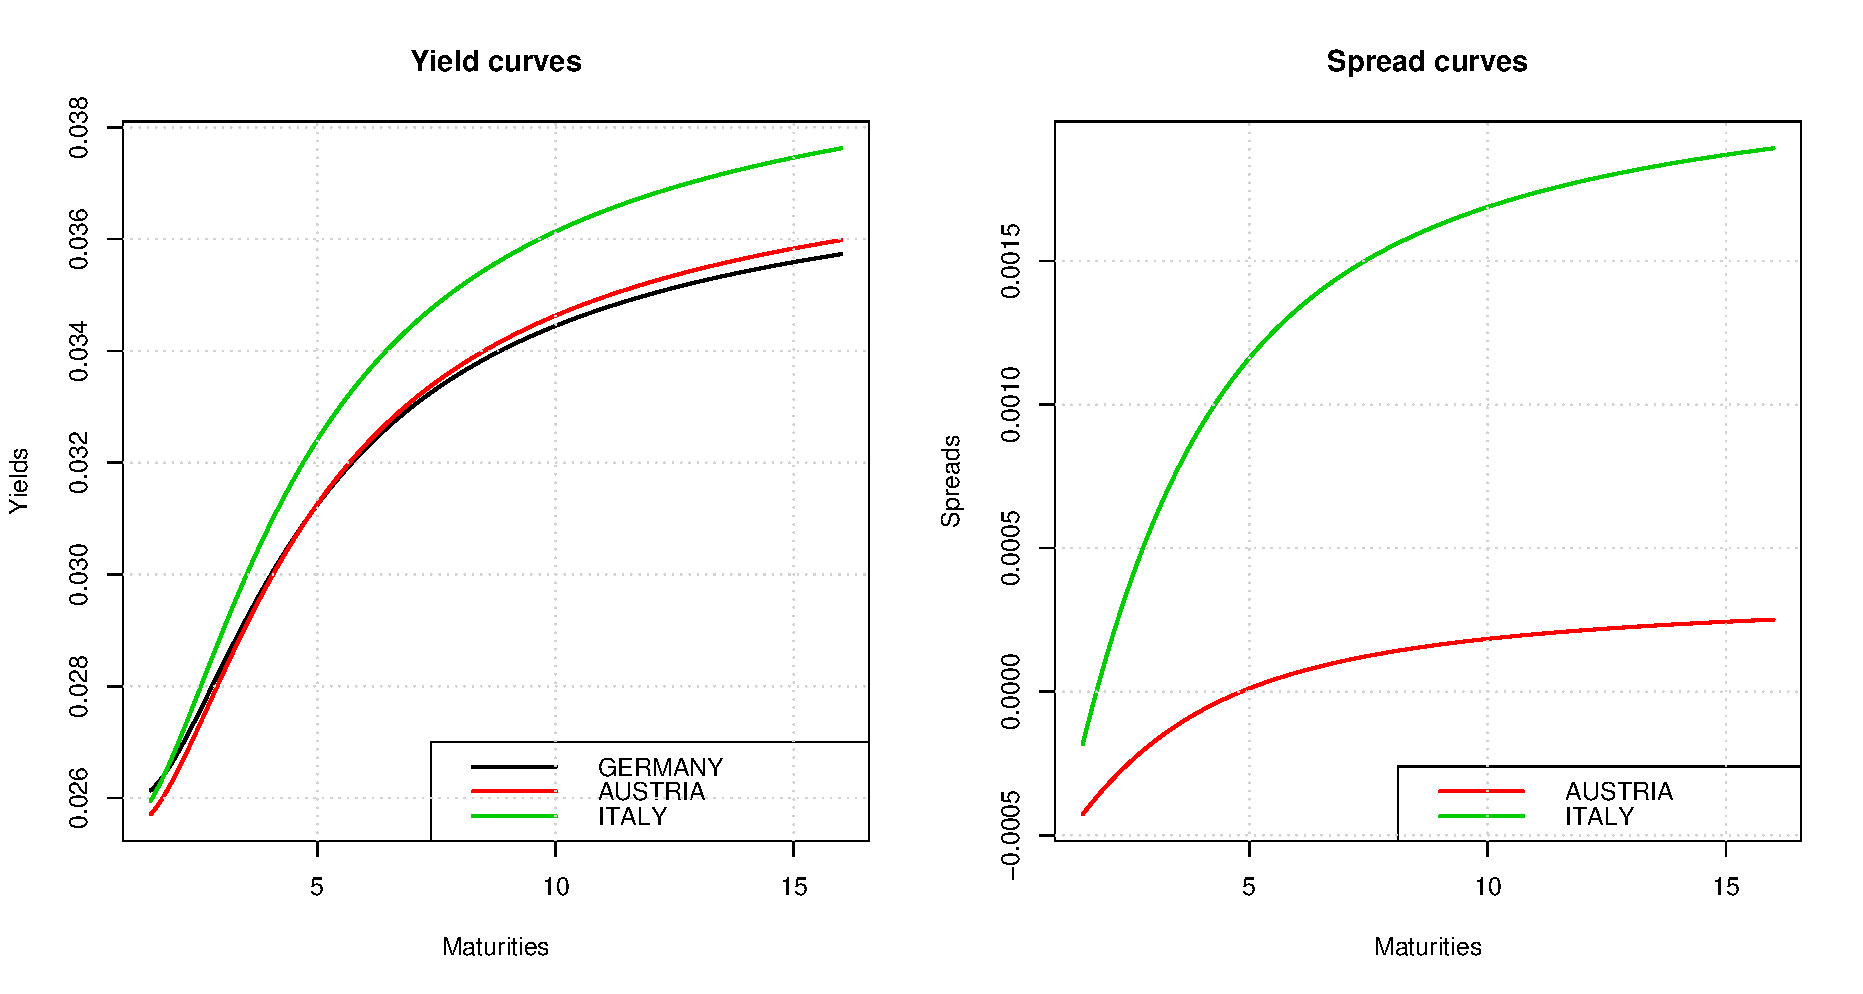
\includegraphics[width=0.97\textwidth]{curves}
%\end{center}
\end{frame}


\begin{frame}
  \frametitle{Nelson and Siegel (1987) approach}
  %\framesubtitle{Untertitel sind optional.}
   \begin{beamerboxesrounded}[shadow=true]{Instantaneous forward rates}
\begin{equation*}
	    f(m,\bm{b}) = \beta_0 + \beta_1 \exp(-\frac{m}{\tau_1}) + \beta_2 \frac{m}{\tau_1} \exp(-\frac{m}{\tau_1})
\end{equation*}
 \end{beamerboxesrounded} 

 \vspace{1.5cm}

\begin{beamerboxesrounded}[shadow=true]{Spot rates}
\begin{equation*}\label{nelson}
    s(m,\bm{b}) = \beta_0 + \beta_1\frac{1-\exp(-\frac{m}{\tau_1})}{\frac{m}{\tau_1}} + \beta_2\left(\frac{1-\exp(-\frac{m}{\tau_1})}{\frac{m}{\tau_1}} - \exp(-\frac{m}{\tau_1})\right)
\end{equation*}
\end{beamerboxesrounded}

%\begin{center}
%	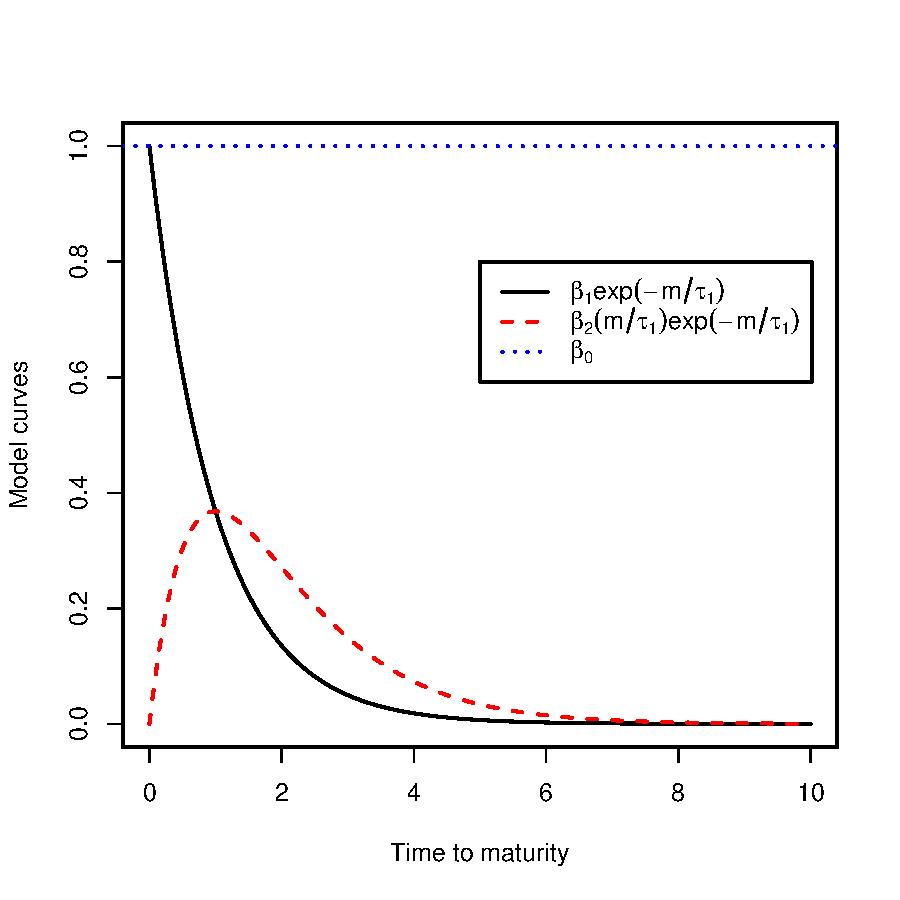
\includegraphics[width=0.65\textwidth]{fignelson}
%\end{center}
\end{frame}


\begin{frame}
  \frametitle{Svensson (1994) approach}
 \begin{itemize}
   \item Svensson (1994) extended the functional form by two additional parameters which allows for a second hump-shape
 \end{itemize}

\begin{beamerboxesrounded}[shadow=true]{Instantaneous forward rates}
\begin{equation*}
	    f(m,\bm{b}) = \beta_0 + \beta_1 \exp(-\frac{m}{\tau_1}) + \beta_2 \frac{m}{\tau_1} \exp(-\frac{m}{\tau_1})+\beta_3 \frac{m}{\tau_2} \exp(-\frac{m}{\tau_2})
\end{equation*}
\end{beamerboxesrounded}
\vspace{0.5cm}
\begin{beamerboxesrounded}[shadow=true]{Spot rates}
\begin{multline*}\label{svspot}
    s(m,\bm{b}) = \beta_0 + \beta_1\frac{1-\exp(-\frac{m}{\tau_1})}{\frac{m}{\tau_1}} + \beta_2\left(\frac{1-\exp(-\frac{m}{\tau_1})}{\frac{m}{\tau_1}} - \exp(-\frac{m}{\tau_1})\right) \\+ \beta_3\left(\frac{1-\exp(-\frac{m}{\tau_2})}{\frac{m}{\tau_2}} - \exp(-\frac{m}{\tau_2})\right)
\end{multline*}
\end{beamerboxesrounded}
\end{frame}

\begin{frame}
	\frametitle{Decomposition of the Svensson forward rate function}
	
	\begin{center}
	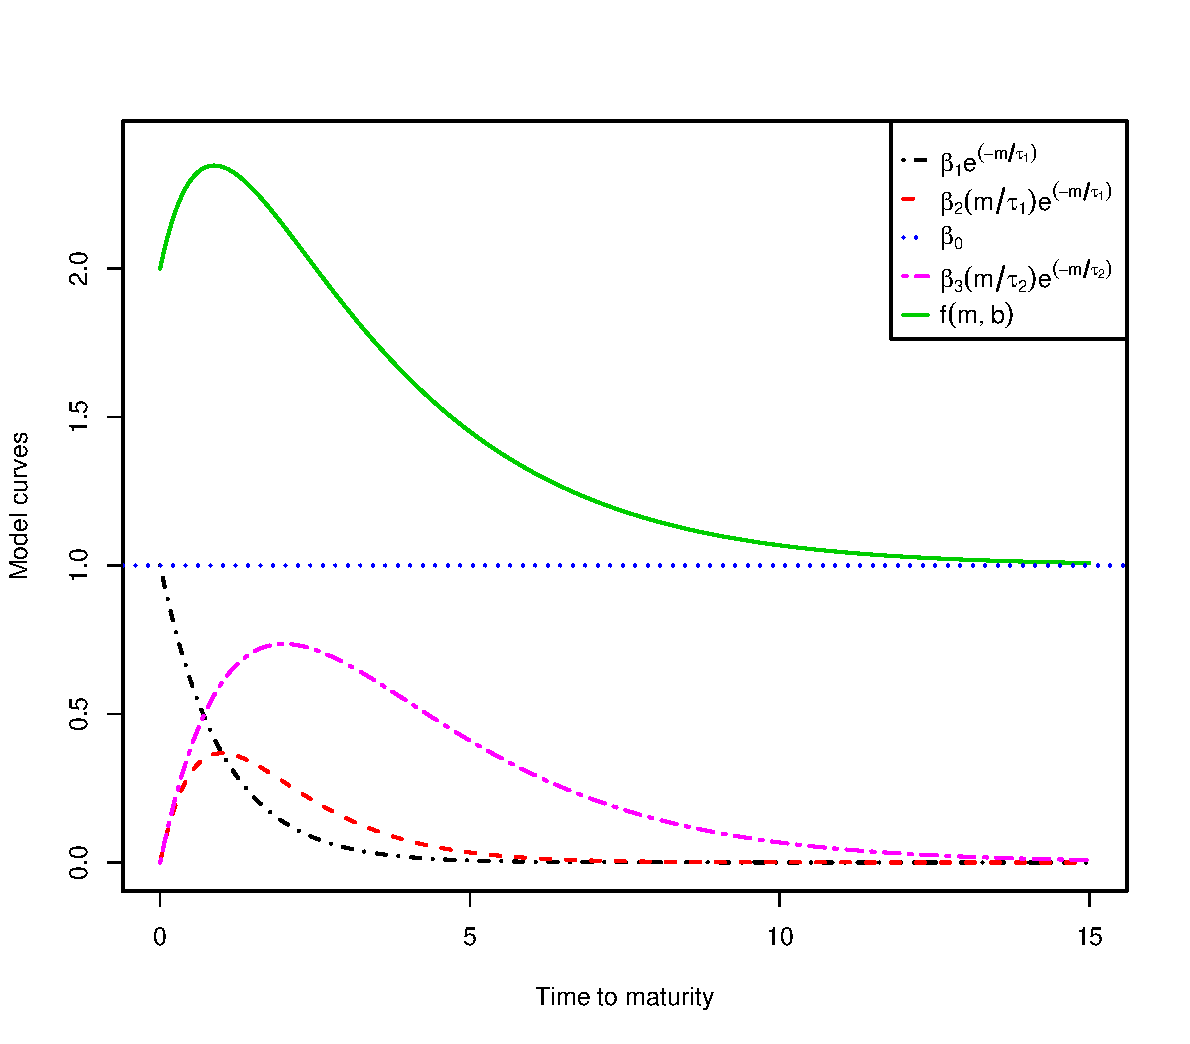
\includegraphics[width=0.8\textwidth]{sv.pdf}
	\end{center}

\end{frame}


\begin{frame}
	\frametitle{Term structure estimation procedure \newline Notation I}
	\begin{beamerboxesrounded}[shadow=true]{Maturity matrix $\bm{M}$}
		\begin{equation*}\label{maturitym}
		\bm{M}_{\left[n\times m\right]} = \{m_{ij}\}
		\end{equation*}
	\end{beamerboxesrounded}
	\vspace{0.3cm}
	\begin{beamerboxesrounded}[shadow=true]{Cashflow matrix $\bm{C}$}
		 \begin{equation*}\label{cashflowm}	
		\bm{C}_{\left[n\times m\right]} = \{c_{ij}\}
		\end{equation*}
	\end{beamerboxesrounded}
	\vspace{0.3cm}
	\begin{beamerboxesrounded}[shadow=true]{Discount factor matrix $\bm{D}$}
		\begin{equation*}\label{discountm}
		\bm{D}_{\left[n\times m\right]} = \{d_{ij}\}; \qquad d_{ij}=e^{-m_{ij}s(m_{ij},\bm{b})}
		\end{equation*}
	\end{beamerboxesrounded}
	\vspace{0.3cm}
	\begin{beamerboxesrounded}[shadow=true]{Clean price vector $\bm{p}^c$}
		 \begin{equation*}\label{pc}
		\bm{p}^c_{\left[1\times m\right]} = \{p^c_j\}
		\end{equation*}
	\end{beamerboxesrounded}	
\end{frame}


\begin{frame}
	\frametitle{Term structure estimation procedure \newline Notation II}
	\begin{beamerboxesrounded}[shadow=true]{Accrued interest vector $\bm{a}$}
		\begin{equation*}\label{a}
		\bm{a}_{\left[1\times m\right]} = \{a_j\}
		\end{equation*}
	\end{beamerboxesrounded}
	\vspace{0.2cm}
	\begin{beamerboxesrounded}[shadow=true]{Dirty price vector $\bm{p}^d$}
		\begin{equation*}\label{pd}
   		\bm{p}^d_{\left[1\times m\right]}= \{p^d_j\}
		\end{equation*}
		\begin{displaymath}
		\bm{p}^d=\bm{p}^c+\bm{a}
		\end{displaymath}
	\end{beamerboxesrounded}
	\vspace{0.2cm}
	\begin{beamerboxesrounded}[shadow=true]{Weights vector $\bm{w}$}
		\begin{equation*}\label{weights}
   		\bm{w}_{\left[1\times m\right]}= \{w_j\}; \qquad   w_j=\frac{\frac{1}{D_j}}{\sum_{i=1}^m\frac{1}{D_i}}
		\end{equation*}
	\end{beamerboxesrounded}	
\end{frame}

\begin{frame}
	\frametitle{Term structure estimation procedure \newline Objective function}

	\begin{itemize}
		\item Minimization of the weighted pricing or yield errors
	\end{itemize}
	\begin{beamerboxesrounded}[shadow=true]{Objective function}
		\begin{equation*}
		 \bm{b}_{opt} = \min_{b}\left(\left(\bm{\iota}_{\left[1 \times n\right]}\left[\bm{C}\cdot\bm{D}\right] - 		\bm{p}^d\right)^2 \bm{w}\bm{\iota}_{\left[m \times 1\right]} \right)
		 \end{equation*}
	\end{beamerboxesrounded}
	
	\begin{itemize}
		\item The parameter vector is subject to constraints ($\beta_0 >0, \tau_1>0, \tau_2>0$)
	\end{itemize}


\end{frame}





\begin{frame}
	\frametitle{Examples}
\end{frame}

\begin{frame}[allowframebreaks]
 \frametitle<presentation>{References}

  \begin{thebibliography}{10}

  \beamertemplatearticlebibitems
  
   \bibitem{BIS2005}
   Bank for International Settlements
   \newblock Zero-coupon yield curves: technical documentation
   \newblock {\em BIS Papers}, No. 25, October 2005
  
  \bibitem{Bolder1999}
   David Bolder, David Streliski
   \newblock Yield Curve Modelling at the Bank of Canada
   \newblock {\em Bank of Canada, Technical Report}, No. 84, 1999
  
    \bibitem{Geyer1999}
   Alois Geyer, Richard Mader
    \newblock Estimation of the Term Structure of Interest Rates - A Parametric Approach
    \newblock {\em OeNB, Working Paper}, No. 37, 1999

\framebreak
  \bibitem{Jankowitsch2004}
    Rainer Jankowitsch, Stefan Pichler
    \newblock Parsimonious Estimation of Credit Spreads
    \newblock {\em The Journal of Fixed Income}, 14(3):49--63, 2004
    
    \bibitem{Nelson1987}
    Charles R. Nelson, Andrew F. Siegel
    \newblock Parsimonious Modeling of Yield Curves
    \newblock {\em The Journal of Business}, 60(4):473--489, 1987
    
    \bibitem{Svensson1994}
    Lars E.O. Svensson
    \newblock Estimating and Interpreting Forward Interest Rates:\\Sweden 1992 -1994
    \newblock {\em National Bureau of Economic Research, \\Technical Report}, No. 4871, 1994

  \end{thebibliography}
\end{frame}

\end{document}
